\chapter{Metodología}
\label{chap:metodologia}
% Redacción 2026-10-04. Evidencia documental: muografia-documentada, 9558099.
% Respaldo de Overleaf: 03_metodologia.pre-redaccion-2026-10-04.tex.bak.
\newcommand{\FiguraPendienteMet}[4]{%
\begin{figure}[htbp]\centering
\IfFileExists{Figuras/#1.pdf}{\includegraphics[width=\linewidth]{Figuras/#1.pdf}}{%
\fbox{\begin{minipage}{0.91\linewidth}\small\raggedright
\textbf{Figura por elaborar por los autores}\par
\textbf{Archivo:} \texttt{\detokenize{#1.pdf}} en \texttt{Figuras}.\par
#4\par\smallskip
\textbf{Entrega:} PDF vectorial y fuente editable. Usar fondo blanco, letra legible a tamaño final, unidades explícitas y colores distinguibles en escala de grises. Exportar sin capturas ni PNG incrustados. Verificar correspondencia con la versión de datos indicada. El PDF reemplazará automáticamente este recuadro.
\end{minipage}}}
\caption[#2]{#2}\label{#3}\end{figure}}

El procedimiento se desarrolló como un estudio computacional de recuperación de imágenes muográficas de baja estadística. Se partió de escenarios volcánicos idealizados cuya geometría y distribución de materiales eran conocidas; se simuló el transporte de muones, se construyeron imágenes angulares y se redujeron sus conteos de forma controlada. Sobre los pares resultantes se entrenaron modelos de aprendizaje profundo y se evaluó su concordancia con referencias de mayor estadística. La salida estudiada fue una imagen de conteos equivalentes: no se realizó una inversión tridimensional de densidad ni una adquisición de campo.

Las figuras metodológicas incorporadas se seleccionaron de la propuesta de los autores por su correspondencia con la implementación y sus fuentes editables~\parencite{propuestaCapitulos2026}. La descripción sigue la dependencia entre etapas: diseño, simulación, preparación de datos, modelo, entrenamiento y evaluación. Los procedimientos se sustentan en la versión documentada del proyecto~\parencite{repositorioMuografia2026}. Los valores de desempeño y el balance de cumplimiento se reservan para el capítulo~\ref{chap:resultados}. La evaluación incluyó el análisis multifracción y local del tercer objetivo, cuyo procedimiento se ejecutó y revisó antes del cierre experimental. La descripción distingue la generación de datos, el entrenamiento al 5\,\% y la evaluación de los mismos pesos con cuatro fracciones de conteo.

\section{Diseño del estudio y secuencia experimental}\label{sec:met-diseno}
\subsection{Alcance y unidades de análisis}
La simulación permitió controlar los materiales y disponer de una referencia común para comparar métodos. Esta elección es coherente con el uso de muones transmitidos para estudiar diferencias de columna de masa, sin identificar la respuesta simulada con la de un instrumento real~\parencite{bonomi2020,lesparre2010}. La representatividad adoptada fue de mecanismos y configuraciones: trayectorias, contrastes de densidad y fluctuaciones de conteo. No se pretendió representar estadísticamente una población de volcanes ni reproducir un sitio particular.

Se distinguieron cuatro unidades. La geometría definió un escenario completo; la vista, una posición de observación; la realización, un submuestreo de una referencia fija; y la ejecución de entrenamiento, una trayectoria de optimización. Esta separación evitó tratar píxeles o realizaciones de una vista como escenarios independientes. Los métodos se compararon sobre las mismas entradas y referencias. Los resúmenes entre escenarios se calcularon por geometría, manteniendo separadas prueba y generalización.

La Tabla~\ref{tab:met-etapas} relaciona las etapas con los objetivos. La Figura~\ref{fig:met-flujo} muestra su secuencia y la separación entre generación de datos, ajuste y evaluación.
\begin{table}[htbp]\centering\small
\caption{Etapas metodológicas y productos del estudio.}\label{tab:met-etapas}
\begin{tabularx}{\linewidth}{@{}>{\raggedright\arraybackslash}p{2.5cm}>{\raggedright\arraybackslash}X>{\raggedright\arraybackslash}X@{}}\toprule
Etapa & Procedimiento & Producto y función\\\midrule
Generación (OE1) & Configurar escenarios, fuente y transporte; consolidar imágenes. & Referencias y pares de conteo verificables.\\
Aprendizaje (OE2) & Transformar datos, entrenar U-Net y cGAN, estudiar ajustes. & Pesos y configuraciones vinculados con sus datos.\\
Evaluación (OE2--OE3) & Comparar similitud, cuentas, contraste y fracciones. & Tablas por escenario y curvas descriptivas.\\\bottomrule
\end{tabularx}\end{table}
\FiguraPendienteMet{met_01_flujo_cerrado}{Secuencia experimental y separación de las particiones.}{fig:met-flujo}{Elaborar un diagrama en dos filas: catálogo y fuente; Geant4; 114 referencias; submuestreo; partición por geometría; escala ajustada solo con entrenamiento; entrenamiento y selección con validación; ocho modelos congelados; evaluación; curvas descriptivas. Separar OE1, OE2 y OE3 con colores. Dibujar una frontera que impida utilizar prueba/generalización para ajustar escala o pesos. Incluir el complemento OE3-C1: mismos ocho pesos entrenados al 5 por ciento, inferencia al 1, 5, 10 y 50 por ciento, métricas locales y criterio conjunto por vista frente a entrada sin red al 50 por ciento. Eliminar toda indicación de objetivo pendiente. Mostrar reutilización del bloque al 5 por ciento. No confundir el entrenamiento con la evaluación multifracción. No incluir resultados ni porcentajes de cumplimiento.}

\subsection{Versiones y condiciones de comparación}
Se utilizó como base final la campaña corregida de la entrega \texttt{f395570}. Las referencias históricas se conservaron como antecedentes; no se convirtieron en datos finales mediante cambios de nombre. Esta distinción fue necesaria porque cambiaron la construcción geométrica, el registro angular y la receta de transporte. La distribución de aprendizaje se vinculó con las referencias finales mediante comprobaciones de contenido.

Se variaron el nivel de conteo, el tipo y contraste de anomalía, la configuración geométrica y la vista. Dentro de cada comparación se conservaron fuente, receta, coordenadas, referencia y preprocesamiento. Las respuestas incluyeron similitud, sesgo de cuentas, error espacial y contraste. Así se distinguió la modificación evaluada de las condiciones mantenidas constantes.

Los ajustes de redes fueron decisiones de desarrollo sobre validación, no ensayos confirmatorios independientes de los resultados que los motivaron. Las escenas reservadas habían sido conocidas en etapas históricas del proyecto. Aunque las redes finales no se ajustaron con esas particiones, su evaluación se presentó como descriptiva sobre un catálogo potencialmente expuesto. La separación de datos en el entrenamiento actual no elimina ese antecedente.

\section{Escenarios y simulación de muones}\label{sec:met-simulacion}
\subsection{Catálogo y asignación de materiales}\label{subsec:met-geometrias}
Se emplearon diecinueve edificios cónicos, con radios basales entre 509,7 y 698,7~m y alturas entre 356,2 y 449,6~m. La roca de fondo tuvo densidad de 2,65~g\,cm$^{-3}$. El control homogéneo fue \texttt{geo-train-01}; los otros dieciocho escenarios incorporaron conductos, cavidades o cuerpos densos. Se representaron mediante cilindros, esferas y elipsoides, respectivamente. La geometría \texttt{geo-gen-01} contuvo un conducto y dos cavidades; no fue el control homogéneo.

Cada escenario conservó dimensiones, posiciones y densidades en una descripción estructurada. Esos parámetros produjeron diferencias de columna de masa y de proyección sin atribuir al catálogo validación geológica externa. La Figura~\ref{fig:met-geometria} permite reconocer primitivas, coordenadas y posiciones de observación.
\begin{figure}[htbp]\centering
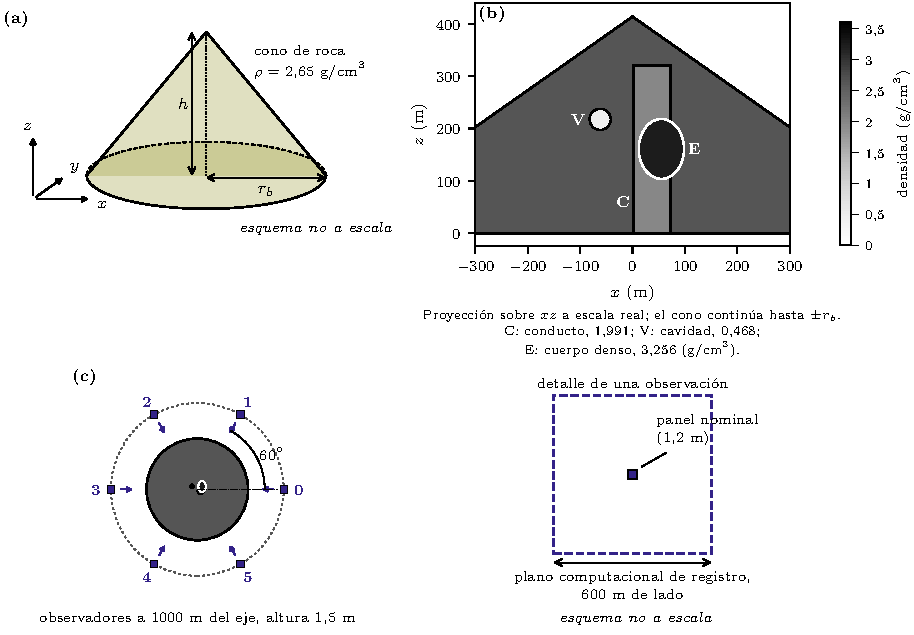
\includegraphics[width=\linewidth]{met_02_escenario_y_vistas.pdf}
\caption[Geometría idealizada y posiciones de observación]{Geometría idealizada y seis posiciones de observación. Se ilustra geo-train-08; las densidades son nominales. El panel de detalle distingue el panel nominal de 1,2 m del plano computacional de 600 m. Fuente: elaboración de los autores, conservada en la propuesta de capítulos.}\label{fig:met-geometria}
\end{figure}

Para resolver las intersecciones se adoptó la prioridad de la última anomalía en el orden del catálogo. La Ecuación~\eqref{eq:met-material} expresa la región asignada a cada material: se restringió la anomalía al edificio y se sustrajeron las anomalías posteriores.
\begin{equation}\mathcal R_i=(A_i\cap\mathcal K)\setminus\bigcup_{j>i}A_j.\label{eq:met-material}\end{equation}
Aquí $A_i$ es la primitiva, $\mathcal K$ el edificio y $\mathcal R_i$ su región final. Se emplearon operaciones booleanas y un margen interior de 1~mm cuando fue necesario recortar contra el edificio, evitando superficies coincidentes. Esta regla no implica identidad matemática de todas las fronteras con el motor analítico. Se conservaron también las diferencias declaradas de densidad del aire. En particular, el constructor conservado sustituyó densidades inferiores a 0,05~g\,cm$^{-3}$ por \texttt{G4\_AIR}. Se distinguieron las densidades nominales del catálogo de la asignación material del transporte; esta distinción se retoma al describir el diagnóstico de opacidad en la sección~\ref{sec:met-opacidad}.

La verificación combinó controles de solapamiento, sondeos de material, comparación de volúmenes e inspección de cortes. Las intersecciones se contrastaron mediante integración independiente. Se distinguió ausencia de advertencias bajo el muestreo aplicado de una prueba universal de navegación. La concordancia geométrica tampoco cuantificó por sí sola el efecto sobre conteos, por lo que se mantuvieron separados los controles geométricos y de transporte.

\subsection{Fuente y observable}\label{subsec:met-fuente}
La fuente combinó pesos angulares derivados del modelo de \textcite{guan2015muonflux} y cuantiles de momento obtenidos con EcoMug~\parencite{pagano2021}. Las tablas y sus huellas se fijaron como entradas de la receta, sin recalcularlas en cada bloque. La fuente híbrida y su extensión angular formaron parte del modelo; no constituyeron una medición local del flujo cósmico.

La generación cubrió un acimut relativo de menos 35 a 35 grados, mientras que la ventana nominal de imagen cubrió de menos 30 a 30 grados. El margen incorporó direcciones adicionales alrededor de la ventana de registro. En elevación se conservaron los pesos tabulados y la extensión documentada en los extremos; los pesos negativos y los centros inferiores a 0,1 grados se anularon. El momento se obtuvo mediante interpolación lineal por tramos de 257 cuantiles en dieciséis bandas de elevación, usando la banda extrema más cercana fuera del dominio tabulado. Esta definición se conservó con las tablas para que una reproducción no sustituyera inadvertidamente el generador por otra distribución.

Se utilizó Geant4~11.4.2, la lista de física FTFP\_BERT y un corte de producción de 1~m~\parencite{agostinelli2003,allison2016}. Se registraron exclusivamente muones primarios. El corte de producción se distinguió del umbral energético de registro, que exigió energía cinética mayor de 3~GeV al cruzar el plano.

Los impactos nominales se muestrearon sobre un panel de 1,2~m de lado. La inyección se situó junto al cono con margen angular de 5 grados; el plano computacional de registro tuvo 600~m de lado. Este plano no representó un instrumento de esa extensión. Su empleo se examinó mediante controles de bordes y fuente ideal, sin convertirlos en una certificación instrumental. La Tabla~\ref{tab:met-receta} identifica la configuración utilizada.
\begin{table}[htbp]\centering\small
\caption{Configuración de la campaña corregida.}\label{tab:met-receta}
\begin{tabularx}{\linewidth}{@{}p{4.7cm}X@{}}\toprule
Componente & Configuración\\\midrule
Geometrías y vistas & 19 escenarios; seis vistas por escenario.\\
Transporte & Geant4 11.4.2; FTFP\_BERT; primarios.\\
Registro & Energía cinética mayor de 3 GeV.\\
Inyección y plano & Panel nominal de 1,2 m; margen de 5 grados; registro de 600 m de lado.\\
Primarios simulados & 344 millones de primarios por vista; nueve bloques.\\
Resolución & 256 filas de elevación y 256 columnas de acimut.\\
Producción & SC3, partición AMD, 64 hilos, 8 GB solicitados por trabajo; GCC 14.2.0.\\\bottomrule
\end{tabularx}\end{table}

\subsection{Número de muones simulados y consolidación}\label{subsec:met-campana}
La campaña final utilizó el mismo número de primarios en cada vista; no se reutilizó el sorteo histórico de eventos asociado a treinta días. Las Ecuaciones~\eqref{eq:met-nvista} y~\eqref{eq:met-ntotal} definen el número de primarios por vista y de toda la campaña. Los bloques se identificaron mediante manifiesto y semillas propias.
\begin{samepage}
\begin{subequations}
\begin{equation}N_{gv}=344\times10^6.\label{eq:met-nvista}\end{equation}
\begin{equation}N_{\mathrm{camp}}=\sum_{g=1}^{19}\sum_{v=0}^{5}N_{gv}=39\,216\,000\,000.\label{eq:met-ntotal}\end{equation}
\end{subequations}
\end{samepage}
Los índices $g$ y $v$ identifican geometría y vista. Primarios generados y detectados no se consideraron equivalentes. Cada bloque produjo histograma y metadatos; para consolidar se exigió compatibilidad de receta, coordenadas e identidad. Se sumaron cuentas enteras, sin promediar ni suavizar.

Las Ecuaciones~\eqref{eq:met-fusion} y~\eqref{eq:met-detectados} definen referencia y total registrado; $b$ recorre bloques, $i$ elevación y $j$ acimut.
\begin{samepage}
\begin{subequations}
\begin{equation}C_{gvij}=\sum_{b=1}^{9}C^{[b]}_{gvij}.\label{eq:met-fusion}\end{equation}
\begin{equation}D_{gv}=\sum_{i=0}^{255}\sum_{j=0}^{255}C_{gvij}\leq N_{gv}.\label{eq:met-detectados}\end{equation}
\end{subequations}
\end{samepage}
Cada píxel representa primarios transmitidos que cumplieron el registro. No representa directamente densidad, opacidad ni transmisión normalizada. La referencia conserva fluctuaciones porque es una realización finita del transporte.

\subsection{Coordenadas y exportación}
Se mantuvo elevación en filas y acimut relativo en columnas. La campaña final utilizó bordes uniformes en acimut y centros uniformes en elevación. Las Ecuaciones~\eqref{eq:met-azedge} y~\eqref{eq:met-azcenter} definen el primer eje; las Ecuaciones~\eqref{eq:met-elcenter} y~\eqref{eq:met-elstep}, el segundo.
\begin{samepage}
\begin{subequations}
\begin{equation}\alpha^e_j=-30^\circ+j\frac{60^\circ}{256},\quad j=0,\ldots,256.\label{eq:met-azedge}\end{equation}
\begin{equation}\alpha_j=\frac{\alpha^e_j+\alpha^e_{j+1}}2,\quad j=0,\ldots,255.\label{eq:met-azcenter}\end{equation}
\begin{equation}\eta_i=2^\circ+i\frac{45^\circ}{255},\quad i=0,\ldots,255.\label{eq:met-elcenter}\end{equation}
\begin{equation}\Delta\eta=\frac{45^\circ}{255}.\label{eq:met-elstep}\end{equation}
\end{subequations}
\end{samepage}
Los bordes de elevación se obtuvieron de puntos medios entre centros, extendiendo medio paso en ambos extremos. El soporte efectivo fue aproximadamente de 1,911765 a 47,088235 grados; describirlo como bordes de 2 a 47 grados habría desplazado medio píxel la correspondencia con los archivos. La elevación se midió desde el horizonte y no se confundió con el ángulo cenital referido a la vertical.

Se exportaron coordenadas explícitas con los conteos; no se reconstruyeron desde una figura. La Figura~\ref{fig:met-malla} explica la relación entre dirección y arreglo. Se verificó correspondencia entre histogramas y matrices, incluyendo coordenadas.
\begin{figure}[htbp]\centering
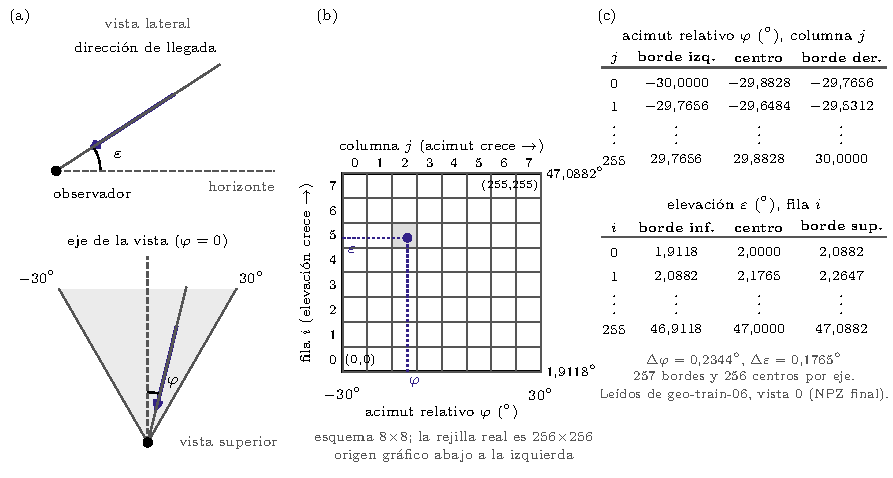
\includegraphics[width=\linewidth]{met_03_malla_angular.pdf}
\caption[Coordenadas y malla angular]{Direcciones, índices y coordenadas angulares. La rejilla simplificada ilustra la orientación; los valores proceden de geo-train-06, vista 0. Fuente: elaboración de los autores.}\label{fig:met-malla}
\end{figure}

\section{Verificación y preparación del conjunto}\label{sec:met-datos}
\subsection{Integridad, bordes y estadística de roca}
Se verificaron presencia y huellas de archivos, compatibilidad de metadatos y conservación de cuentas y coordenadas. Después se examinaron aspectos del observable. La integridad acreditó identidad de archivos, mientras que los controles del modelo acotaron su interpretación; ninguna verificación sustituyó a las demás.

Para el borde angular se compararon probabilidades registradas con una referencia ideal de la fuente. Las Ecuaciones~\eqref{eq:met-residuo} y~\eqref{eq:met-diferencia} definen residuo y diferencia respecto de una región de referencia. $K_{gvr}$ es el conteo regional y $p_r^{\mathrm{ideal}}$ y $p_r^{\mathrm{nom}}$ son las probabilidades ideal y nominal conservadas en el contrato.
\begin{samepage}
\begin{subequations}
\begin{equation}e_{gvr}=\frac{K_{gvr}/N_{gv}-p_r^{\mathrm{ideal}}}{p_r^{\mathrm{nom}}}.\label{eq:met-residuo}\end{equation}
\begin{equation}d_{gvr}=e_{gvr}-e_{gvr_0}.\label{eq:met-diferencia}\end{equation}
\end{subequations}
\end{samepage}
Se definieron quince regiones de borde por vista: cinco columnas en cada extremo azimutal, restringidas al cielo entre 30 y 42 grados de elevación, y las cinco filas superiores. La región interior de referencia utilizó cielo en el mismo intervalo de elevación, excluyendo veinte columnas por cada lado. Así se contrastaron bordes con interior bajo la misma fuente, sin exigir uniformidad de cuentas entre elevaciones.

Se construyeron intervalos con cobertura familiar del 95\,\% bajo el modelo binomial definido en la receta, frente a tolerancia de un punto porcentual. Se conservaron máscaras, referencia ideal y procedimiento de cálculo versionado. El control acotó el comportamiento del observable en bordes; no certificó la respuesta de un instrumento.

Para precisar el cálculo se emplearon límites binomiales Clopper--Pearson y corrección de Bonferroni. La Ecuación~\eqref{eq:met-alpha} define el nivel individual: el factor 16 incluye quince regiones de borde y el interior, y el factor 114 incluye todas las vistas. Las Ecuaciones~\eqref{eq:met-cplow} y~\eqref{eq:met-cphigh} especifican los extremos para un conteo regional $K$ en $N$ primarios; $B^{-1}$ denota un cuantil beta.
\begin{samepage}
\begin{subequations}
\begin{equation}\alpha_* = \frac{0{,}05}{114\times16}.\label{eq:met-alpha}\end{equation}
\begin{equation}a_r=\begin{cases}0,&K=0,\\ B^{-1}(\alpha_*/2;K,N-K+1),&K>0.\end{cases}\label{eq:met-cplow}\end{equation}
\begin{equation}b_r=\begin{cases}1,&K=N,\\ B^{-1}(1-\alpha_*/2;K+1,N-K),&K<N.\end{cases}\label{eq:met-cphigh}\end{equation}
\end{subequations}
\end{samepage}
Al transformar los extremos con la Ecuación~\eqref{eq:met-residuo} se obtuvieron límites para cada residuo. La Ecuación~\eqref{eq:met-intervalo} define el intervalo conservador de la diferencia; la Ecuación~\eqref{eq:met-aceptacion} expresa su criterio de conformidad.
\begin{samepage}
\begin{subequations}
\begin{equation}I_{gvr}=[e^-_{gvr}-e^+_{gvr_0},\ e^+_{gvr}-e^-_{gvr_0}].\label{eq:met-intervalo}\end{equation}
\begin{equation}I_{gvr}\subseteq[-0{,}01;\,0{,}01].\label{eq:met-aceptacion}\end{equation}
\end{subequations}
\end{samepage}
Se exigió que todo el intervalo estuviera dentro de la tolerancia; no bastó el estimador puntual. La cobertura familiar se sostuvo bajo el modelo binomial marginal, sin exigir independencia entre regiones. No incluyó incertidumbre de las hipótesis físicas de la fuente ideal.

La estadística de roca se examinó en regiones de $4\times4$ píxeles, seleccionadas por columna nominal de cono homogéneo entre 30\,000 y 100\,000~g\,cm$^{-2}$. Las Ecuaciones~\eqref{eq:met-roca} y~\eqref{eq:met-fraccion-roca} definen conteo y proporción de regiones con al menos cien cuentas.
\begin{samepage}
\begin{subequations}
\begin{equation}H_{gvq}=\sum_{(i,j)\in q}C_{gvij}.\label{eq:met-roca}\end{equation}
\begin{equation}F_{gv}=\frac1{|\mathcal Q_{gv}|}\sum_{q\in\mathcal Q_{gv}}\mathbf1\{H_{gvq}\geq100\}.\label{eq:met-fraccion-roca}\end{equation}
\end{subequations}
\end{samepage}
$\mathcal Q_{gv}$ contiene las regiones elegibles. La meta descriptiva se fijó en una proporción mínima de 0,90 y se aplicó a este soporte; no caracterizó toda la roca ni cada píxel. Las vistas que no alcanzaron la meta se conservaron como excepciones, sin eliminarlas del aprendizaje o evaluación. Su balance pertenece a resultados.

\subsection{Construcción de pares}\label{subsec:met-pares}
La estadística se redujo conservando cada evento de referencia con probabilidad $f$, sin simular una nueva campaña para cada fracción. Se utilizaron 0,50, 0,10, 0,05 y 0,01, con veinte realizaciones por vista y fracción. Las Ecuaciones~\eqref{eq:met-binomial}, \eqref{eq:met-media} y~\eqref{eq:met-varianza} definen el muestreo y sus momentos condicionales~\parencite{kingman1992}.
\begin{samepage}
\begin{subequations}
\begin{equation}L^{(f,k)}_{gvij}\mid C_{gvij}\sim\operatorname{Binomial}(C_{gvij},f).\label{eq:met-binomial}\end{equation}
\begin{equation}\mathbb E[L^{(f,k)}_{gvij}\mid C_{gvij}]=fC_{gvij}.\label{eq:met-media}\end{equation}
\begin{equation}\operatorname{Var}[L^{(f,k)}_{gvij}\mid C_{gvij}]=f(1-f)C_{gvij}.\label{eq:met-varianza}\end{equation}
\end{subequations}
\end{samepage}
La referencia y las entradas comparten eventos de origen. Las semillas se derivaron de la maestra 20260805 y de índices de geometría, vista, fracción y realización. Se conservaron los estados y se reprodujo contenido con la versión registrada de NumPy~\parencite{harris2020}. El empaquetado final no aplicó suavizado, normalización por imagen ni recorte a 65\,535 cuentas; no se confundió con la implementación histórica que incluía ese recorte.

El Algoritmo~\ref{alg:met-pares} sintetiza el procedimiento. La Figura~\ref{fig:met-pares} ilustrará sus productos con datos identificados de la campaña final.
\begin{algorithm}[htbp]\small
\caption{Construcción reproducible de pares.}\label{alg:met-pares}
\begin{algorithmic}[1]
\Require Referencias verificadas, coordenadas, fracciones y semilla maestra.
\Ensure Pares y metadatos vinculados con sus referencias.
\For{cada geometría y vista en el orden fijado}
\State Verificar identidad, forma y coordenadas.
\For{cada fracción y cada una de las veinte realizaciones}
\State Derivar un estado aleatorio a partir de los índices registrados.
\State Muestrear cada píxel mediante la Ecuación~\eqref{eq:met-binomial}.
\State Conservar los conteos y asociarlos con la referencia.
\EndFor
\State Guardar coordenadas, fracciones, semillas y huellas de contenido.
\State Comprobar correspondencia con los arreglos originales.
\EndFor
\end{algorithmic}\end{algorithm}
\begin{figure}[htbp]\centering
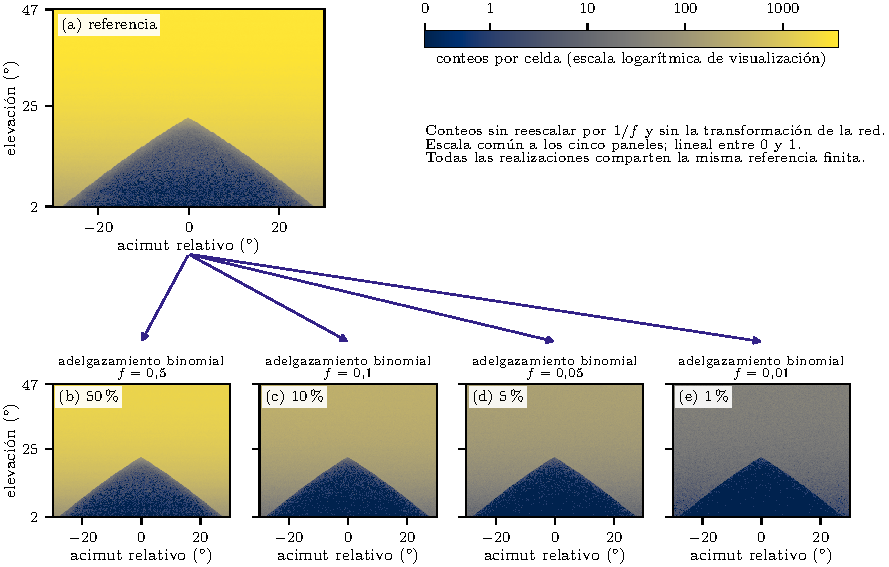
\includegraphics[width=\linewidth]{met_04_pares_conteo.pdf}
\caption[Referencia y pares de conteo]{Referencia finita y cuatro realizaciones reducidas de geo-train-06, vista 3, realización 0. Se muestran conteos sin dividir por la fracción, con escala común logarítmica de visualización, lineal entre cero y una cuenta. Fuente: elaboración de los autores.}\label{fig:met-pares}
\end{figure}

\subsection{Particiones y contrato de datos}\label{subsec:met-particiones}
Se asignaron geometrías completas a entrenamiento, validación, prueba y generalización. Sus vistas, fracciones y realizaciones permanecieron juntas, evitando compartir referencias entre ajuste y evaluación~\parencite{kaufman2012}. La Tabla~\ref{tab:met-particiones} distingue el conjunto completo del utilizado al 5\,\%.
\begin{table}[htbp]\centering\small
\caption{Escenarios, vistas y pares por partición.}\label{tab:met-particiones}
\begin{tabular}{@{}lrrrr@{}}\toprule
Partición & Geometrías & Vistas & Pares totales & Pares al 5\,\%\\\midrule
Entrenamiento & 12 & 72 & 5\,760 & 1\,440\\
Validación & 3 & 18 & 1\,440 & 360\\
Prueba & 3 & 18 & 1\,440 & 360\\
Generalización & 1 & 6 & 480 & 120\\\midrule
Total & 19 & 114 & 9\,120 & 2\,280\\\bottomrule
\end{tabular}\end{table}
No se reasignaron casos después de observar su dificultad. La única geometría de generalización permitió estudiar un caso separado, sin estimar variabilidad entre varios escenarios de esa partición. El lector de entrenamiento aceptó únicamente train y val; la evaluación final utilizó otro contrato, con pesos y archivos identificados.

La conversión a la distribución de aprendizaje se verificó contra cada paquete de origen. Se conservaron huellas de archivo y de contenido cuando fue necesario distinguir compresión y arreglos. Una igualdad de contenido no autorizó sustituir archivos dentro de un manifiesto congelado: otra distribución requirió identidad y procedencia propias.


\section{Representación de conteos y arquitectura}\label{sec:met-modelo}
\subsection{Normalización disponible en inferencia}\label{subsec:met-preprocesamiento}
Los conteos se transformaron para estabilizar la representación y obtener una salida compatible con sigmoide. Se fijó una escala con el máximo de las referencias de entrenamiento, sin usar máximos de validación o reservas. Las Ecuaciones~\eqref{eq:met-max} y~\eqref{eq:met-escala} definen el ajuste.
\begin{samepage}
\begin{subequations}
\begin{equation}M=\max_{g\in\mathcal G_{\mathrm{train}},v,i,j}C_{gvij}=3786.\label{eq:met-max}\end{equation}
\begin{equation}s=\log(1+\max\{1,M\})=8{,}239329427901795.\label{eq:met-escala}\end{equation}
\end{subequations}
\end{samepage}
La escala se guardó con contrato y pesos. La entrada se corrigió por su fracción conocida antes de transformarla, expresándola en cuentas equivalentes a la referencia. Las Ecuaciones~\eqref{eq:met-transformacion}, \eqref{eq:met-entrada} y~\eqref{eq:met-objetivo} se aplicaron elemento a elemento.
\begin{samepage}
\begin{subequations}
\begin{equation}T_s(c)=\frac{\log(1+c)}{s+\log(1+c)},\quad c\geq0.\label{eq:met-transformacion}\end{equation}
\begin{equation}\boldsymbol u=T_s(\boldsymbol L/f).\label{eq:met-entrada}\end{equation}
\begin{equation}\boldsymbol y=T_s(\boldsymbol C).\label{eq:met-objetivo}\end{equation}
\end{subequations}
\end{samepage}
La entrada depende de sus conteos, de $f$ y de una escala fijada previamente; no necesita la referencia de alta estadística de esa vista. Una entrada vacía produce ceros. No se supuso amplitud transformada proporcional a $f$, pues la transformación es no lineal.

Las cuentas se recuperaron mediante la Ecuación~\eqref{eq:met-inversa}. Una predicción fuera del dominio invertible se trató como incidencia explícita, sin recortes silenciosos.
\begin{equation}T_s^{-1}(z)=\exp\left(\frac{sz}{1-z}\right)-1,\quad 0\leq z<1.\label{eq:met-inversa}\end{equation}
Un error pequeño en la representación acotada no equivale a un error constante en cuentas; se evaluaron ambos dominios. La Figura~\ref{fig:met-normalizacion} muestra esa separación.
\begin{figure}[htbp]\centering
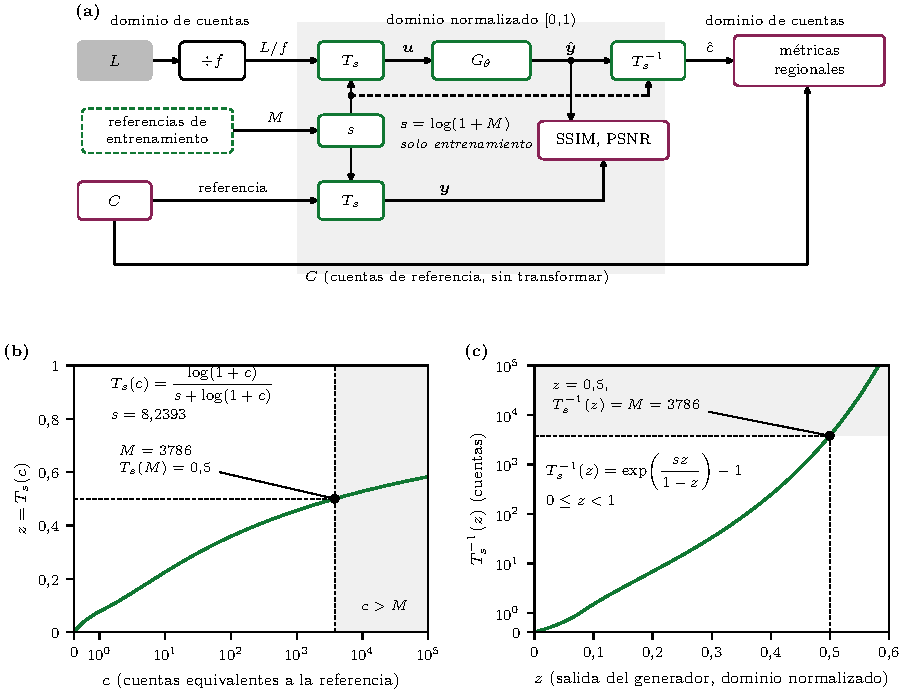
\includegraphics[width=\linewidth]{met_05_normalizacion.pdf}
\caption[Normalización y recuperación de cuentas]{Transformación de entrada y referencia y recuperación de cuentas equivalentes. La escala procede exclusivamente de entrenamiento; los gráficos representan la transformación y su inversa. Fuente: elaboración de los autores.}\label{fig:met-normalizacion}
\end{figure}

\subsection{Generador y crítico}
El generador se basó en U-Net, con codificador y decodificador conectados a iguales resoluciones~\parencite{ronneberger2015}. Las concatenaciones combinaron información espacial temprana con representaciones de mayor contexto. La implementación \texttt{unet\_dc\_5} tuvo cinco niveles con canales 64, 128, 256, 512 y 512. Cada bloque incluyó dos convoluciones de $3\times3$, normalización por instancia y LeakyReLU. Cuatro reducciones llevaron la imagen de $256\times256$ a $16\times16$; el decodificador recuperó resolución mediante convoluciones transpuestas. Una convolución de $1\times1$ y una sigmoide produjeron un canal.

La Tabla~\ref{tab:met-generador} resume el codificador. La Figura~\ref{fig:met-red} representa además decodificador y crítico. El generador completo tuvo 20\,543\,809 parámetros. La reducción se realizó mediante agrupamiento máximo de $2\times2$. Las convoluciones transpuestas tuvieron núcleo de $2\times2$ y paso dos; cada concatenación se procesó con un bloque de dos convoluciones. La pendiente negativa de LeakyReLU fue 0,2. En el decodificador se recuperaron sucesivamente 512, 256, 128 y 64 canales antes de la proyección final.
\begin{table}[htbp]\centering\small
\caption{Niveles del codificador del generador.}\label{tab:met-generador}
\begin{tabular}{@{}lrr@{}}\toprule
Nivel & Resolución & Canales\\\midrule
Entrada & $256\times256$ & 1\\
Primer bloque & $256\times256$ & 64\\
Segundo bloque & $128\times128$ & 128\\
Tercer bloque & $64\times64$ & 256\\
Cuarto bloque & $32\times32$ & 512\\
Nivel profundo & $16\times16$ & 512\\\bottomrule
\end{tabular}\end{table}
El crítico recibió la entrada junto con una imagen real o generada~\parencite{isola2017}. La concatenación se realizó sobre el eje de canales, formando una entrada de dos canales. Se emplearon cinco convoluciones de núcleo $4\times4$ y relleno de un píxel, con canales de salida 64, 128, 256, 512 y uno. Sus pasos fueron dos, dos, dos, uno y uno. Se aplicaron normalización por instancia en las capas intermedias y LeakyReLU de pendiente 0,2, sin normalización en la primera ni activación sigmoide en la última. Para entrada de $256\times256$, la salida fue de $30\times30$ puntuaciones. El campo receptivo convolucional nominal fue de $70\times70$ píxeles; esta dimensión arquitectónica no se interpretó como resolución física.

La variante \texttt{patch\_critic\_70} produjo puntuaciones espaciales, agregadas por muestra según la Ecuación~\eqref{eq:met-critico}. $P_D$ es el número de parches y $D_{\phi,p}$ su puntuación.
\begin{equation}S_\phi(\boldsymbol u,\boldsymbol y)=\frac1{P_D}\sum_{p=1}^{P_D}D_{\phi,p}(\boldsymbol u,\boldsymbol y).\label{eq:met-critico}\end{equation}
\begin{figure}[htbp]\centering
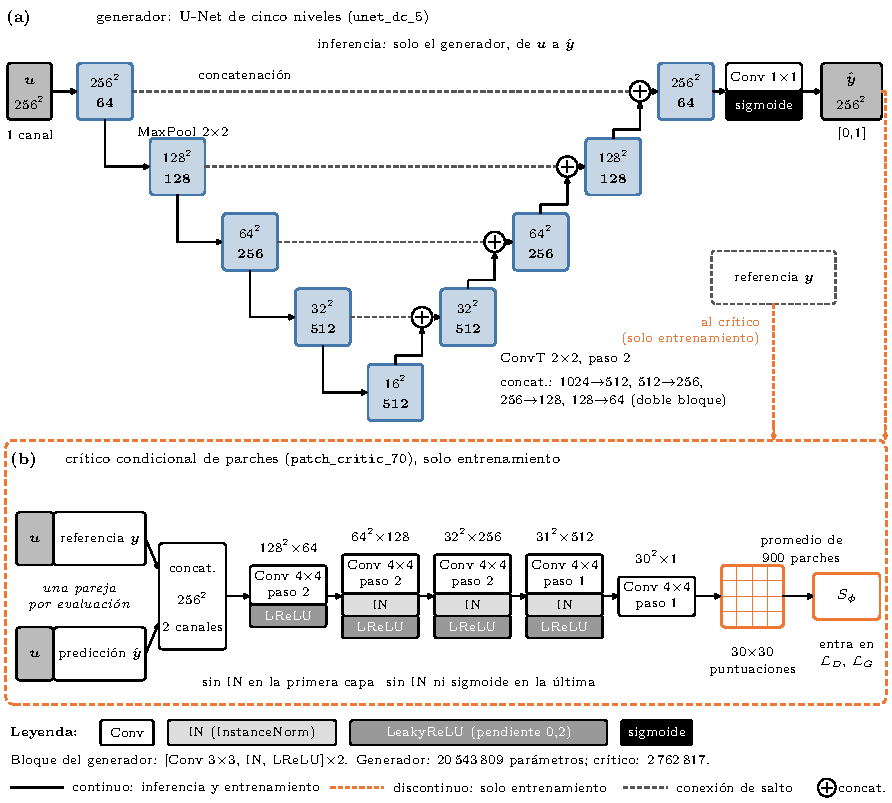
\includegraphics[width=\linewidth]{met_06_generador_critico.pdf}
\caption[Generador U-Net y crítico condicional]{Arquitectura del generador U-Net y del crítico condicional. Se distinguen concatenación de características y promedio de puntuaciones. En inferencia se utiliza solo el generador. Fuente: elaboración de los autores.}\label{fig:met-red}
\end{figure}

\subsection{Pérdidas y coherencia del gradiente}
Se utilizó entrenamiento de Wasserstein con penalización de gradiente~\parencite{gulrajani2017}. Las Ecuaciones~\eqref{eq:met-interpolacion} y~\eqref{eq:met-gp} definen interpolación y penalización. $\epsilon$ se muestreó uniformemente entre cero y uno para cada muestra del lote.
\begin{samepage}
\begin{subequations}
\begin{equation}\widetilde{\boldsymbol y}=\epsilon\boldsymbol y+(1-\epsilon)G_\theta(\boldsymbol u).\label{eq:met-interpolacion}\end{equation}
\begin{equation}\mathcal L_{\mathrm{GP}}=\mathbb E\left[\left(\|\nabla_{\widetilde{\boldsymbol y}}S_\phi(\boldsymbol u,\widetilde{\boldsymbol y})\|_2-1\right)^2\right].\label{eq:met-gp}\end{equation}
\end{subequations}
\end{samepage}
Se diferenció la misma puntuación media que intervino en el término adversario. No se empleó una suma de parches en la penalización ni se dividió el gradiente individual por el tamaño del lote. Se mantuvo así coherencia entre función optimizada y restricción.

Las Ecuaciones~\eqref{eq:met-ld}, \eqref{eq:met-l1} y~\eqref{eq:met-lg} describen pérdidas de crítico, reconstrucción y generador. $P$ es el número de píxeles; las esperanzas se estimaron mediante promedios del lote.
\begin{samepage}
\begin{subequations}
\begin{equation}\mathcal L_D=\mathbb E[S_\phi(\boldsymbol u,G_\theta(\boldsymbol u))]-\mathbb E[S_\phi(\boldsymbol u,\boldsymbol y)]+10\mathcal L_{\mathrm{GP}}.\label{eq:met-ld}\end{equation}
\begin{equation}\mathcal L_1=\mathbb E\left[\frac1P\sum_{p=1}^{P}|G_\theta(\boldsymbol u)_p-y_p|\right].\label{eq:met-l1}\end{equation}
\begin{equation}\mathcal L_G=-\mathbb E[S_\phi(\boldsymbol u,G_\theta(\boldsymbol u))]+100\mathcal L_1.\label{eq:met-lg}\end{equation}
\end{subequations}
\end{samepage}
La U-Net de comparación conservó el generador y minimizó únicamente $100\mathcal L_1$. La igualdad de épocas no implicó igualdad de tiempo de cómputo, pues la cGAN requirió actualizaciones del crítico.

\section{Entrenamiento y desarrollo experimental}\label{sec:met-entrenamiento}
\subsection{Piloto y selección con validación}
Los modelos iniciales se entrenaron desde cero al 5\,\%, con 1\,440 pares de entrenamiento y 360 de validación. Se desactivaron aumentos y nuevos adelgazamientos; las realizaciones permanecieron congeladas. La Tabla~\ref{tab:met-entrenamiento} resume la configuración.
\begin{table}[htbp]\centering\small
\caption{Configuración común del piloto y diferencias entre métodos.}\label{tab:met-entrenamiento}
\begin{tabularx}{\linewidth}{@{}p{3.8cm}XX@{}}\toprule
Parámetro & U-Net & cGAN\\\midrule
Fracción y lote & 0,05; cuatro imágenes & 0,05; cuatro imágenes\\
Optimizador & Adam & Adam para G y D\\
Tasa y betas & $10^{-4}$; $(0;0,9)$ & $10^{-4}$; $(0;0,9)$\\
Semilla & 2026100301 & 2026100301\\
Actualización por lote & Una de G & Cinco de D y una de G\\
Límite de entrenamiento & Hasta 30 épocas & Hasta 30 épocas\\
Selección & Máximo SSIM de validación & Máximo SSIM de validación\\
Parada & Ocho validaciones sin mejora mínima de 0,001 & El mismo criterio\\\bottomrule
\end{tabularx}\end{table}
Se separó el máximo de SSIM para conservar pesos del umbral usado para paciencia. Así no se descartó un máximo real por ser menor que el incremento mínimo de parada. Se distinguió la duración de cada ejecución de la época correspondiente a los pesos seleccionados. El criterio de parada limitó la ejecución, mientras que el máximo de validación determinó el estado utilizado posteriormente; los valores obtenidos se presentan en el capítulo~\ref{chap:resultados}.

Antes de prolongar ejecuciones se comprobó recuperación tras interrupción, conservando redes, optimizadores, estados aleatorios, configuración y contrato. Se rechazaron identidades incompatibles. El Algoritmo~\ref{alg:met-entrenamiento} describe la secuencia adversaria.
\begin{algorithm}[htbp]\small
\caption{Entrenamiento condicional y selección con validación.}\label{alg:met-entrenamiento}
\begin{algorithmic}[1]
\Require Datos train/val verificados, escala, configuración y semilla.
\Ensure Pesos seleccionados, estado recuperable y registro por época.
\State Inicializar G, D y optimizadores, o recuperar un estado compatible.
\For{cada época hasta el límite de épocas o condición de parada}
\For{cada lote de entrenamiento}
\State Transformar entrada y referencia con la escala fija.
\For{cinco actualizaciones del crítico}
\State Generar imágenes sin actualizar G; formar interpolaciones.
\State Calcular puntuaciones y penalización; actualizar D.
\EndFor
\State Calcular reconstrucción y término adversario; actualizar G.
\EndFor
\State Evaluar validación completa sin actualizar parámetros.
\State Conservar máximo de SSIM y actualizar por separado la paciencia.
\State Guardar estado completo e identidad.
\EndFor
\end{algorithmic}\end{algorithm}

\subsection{Ajustes regionales y espaciales}
Los diagnósticos en validación motivaron continuaciones para examinar conservación de cuentas. Se estudió un término regional en U-Net y cGAN y, posteriormente, un término espacial de borde. Estas etapas fueron desarrollo sobre validación; no se convirtieron en réplicas independientes ni se supuso que C0 y C1 definieran siempre lo mismo.

Las Ecuaciones~\eqref{eq:met-media-reg} y~\eqref{eq:met-error-reg} definen media espacial y discrepancia regional. La Ecuación~\eqref{eq:met-lreg} asigna igual peso a familias no vacías y regiones de cada familia, seguido del promedio entre imágenes del lote.
\begin{samepage}
\begin{subequations}
\begin{equation}\overline c_R=\frac1{|R|}\sum_{p\in R}c_p.\label{eq:met-media-reg}\end{equation}
\begin{equation}\ell_R=|\log(1+\overline{\widehat c}_R)-\log(1+\overline c_R)|.\label{eq:met-error-reg}\end{equation}
\begin{equation}\mathcal L_{\mathrm{reg}}=\frac1B\sum_{b=1}^{B}\frac1{|\mathcal F_b|}\sum_{h\in\mathcal F_b}\frac1{|\mathcal R_{bh}|}\sum_{R\in\mathcal R_{bh}}\ell_R.\label{eq:met-lreg}\end{equation}
\end{subequations}
\end{samepage}
$\mathcal F_b$ contiene familias elegibles y $\mathcal R_{bh}$ sus regiones. Se promediaron cuentas antes del logaritmo; promediar logaritmos por píxel habría definido otra función. La implementación evaluó establemente las sumas necesarias.

El ensayo E1 añadió discrepancia absoluta en la máscara de borde mediante la Ecuación~\eqref{eq:met-lborde}. Se rechazaron soportes menores de veinte píxeles, referencias nulas y valores no finitos.
\begin{equation}\mathcal L_{\mathrm{borde}}=\frac1B\sum_{b=1}^{B}\frac{\sum_{p\in R_b}|\widehat c_{bp}-c_{bp}|}{\sum_{p\in R_b}c_{bp}}.\label{eq:met-lborde}\end{equation}
Las Ecuaciones~\eqref{eq:met-c0} y~\eqref{eq:met-c1} definen las ramas de E1: C0 ya incorporó el término regional y C1 añadió el espacial.
\begin{samepage}
\begin{subequations}
\begin{equation}\mathcal L_G^{C0}=\mathcal L_G+\mathcal L_{\mathrm{reg}}.\label{eq:met-c0}\end{equation}
\begin{equation}\mathcal L_G^{C1}=\mathcal L_G^{C0}+0{,}629\mathcal L_{\mathrm{borde}}.\label{eq:met-c1}\end{equation}
\end{subequations}
\end{samepage}
El coeficiente 0,629 se fijó mediante un perfil de gradientes de doce lotes de entrenamiento antes de comparar nuevos resultados de validación. Fue una escala de optimización, no una tolerancia física. Las parejas B1, B2 y B3 usaron semillas 2026100411, 2026100412 y 2026100413. Partieron de los mismos pesos de generador y crítico, con optimizadores nuevos, tasa $10^{-5}$ y cinco épocas adicionales. Se conservó la quinta época, sin seleccionar retrospectivamente una semilla favorable.

La recuperación se examinó también en procesos separados. La corrección CG-04c separó la derivación de Wasserstein y penalización, sumando gradientes antes de un único paso del optimizador, sin cambiar la pérdida. Las comprobaciones correspondieron al entorno entregado, sin atribuir determinismo universal entre plataformas.

La Figura~\ref{fig:met-ensayos} organiza la secuencia. Las máscaras orientaron pérdidas durante entrenamiento, pero no fueron entradas adicionales necesarias para predecir.
\begin{figure}[htbp]\centering
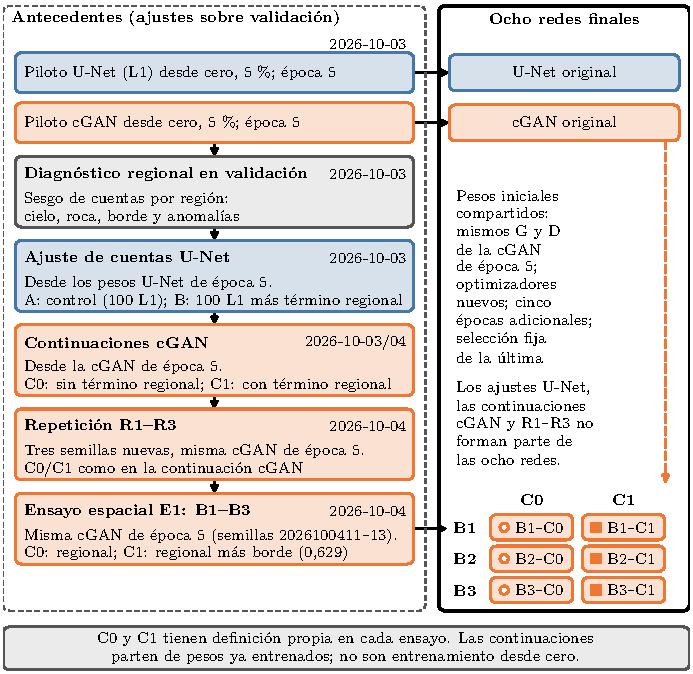
\includegraphics[width=\linewidth]{met_07_secuencia_ensayos.pdf}
\caption[Secuencia de ensayos y modelos finales]{Secuencia de desarrollo y ocho redes finales. La mención de época 5 identifica los pesos seleccionados de los modelos originales, no la duración de sus entrenamientos. C0 y C1 conservan definiciones propias de cada ensayo. Fuente: elaboración de los autores.}\label{fig:met-ensayos}
\end{figure}


\section{Evaluación de similitud y conservación de cuentas}\label{sec:met-evaluacion}
\subsection{Congelamiento e inferencia}
La evaluación final incluyó U-Net y cGAN originales y las seis continuaciones E1. Se añadió la entrada sin red, corregida por fracción y transformada con la misma escala. Pesos y archivos reservados se fijaron mediante huellas antes del cálculo de desempeño. No se sustituyeron pesos según el resultado de prueba.

Cada red se aplicó a 360 entradas de prueba y 120 de generalización, siempre al 5\,\%, en modo evaluación y sin optimización. Se conservaron 120 predicciones por geometría, vinculadas con pesos, datos, escala y orden de muestras. Se verificaron forma, rango y valores finitos. La reevaluación completa de métricas desde matrices conservadas se distinguió de una nueva inferencia: la comparación adicional CPU/GPU utilizó una muestra de treinta y dos imágenes.

\subsection{Métricas de imagen}
Se calcularon SSIM y PSNR en representación acotada y rango uno. Las Ecuaciones~\eqref{eq:met-mse} y~\eqref{eq:met-psnr} definen error cuadrático y transformación a decibelios; $p$ recorre referencia $\boldsymbol y$ y predicción $\boldsymbol z$.
\begin{samepage}
\begin{subequations}
\begin{equation}\operatorname{MSE}=\frac1P\sum_{p=1}^{P}(z_p-y_p)^2.\label{eq:met-mse}\end{equation}
\begin{equation}\operatorname{PSNR}=-10\log_{10}(\operatorname{MSE}).\label{eq:met-psnr}\end{equation}
\end{subequations}
\end{samepage}
Un error nulo se registró como coincidencia perfecta con PSNR infinito, no como cero. SSIM comparó luminancia, contraste y estructura local~\parencite{wang2004}. La Ecuación~\eqref{eq:met-ssim} emplea medias, varianzas y covarianza en ventanas uniformes de $7\times7$. Las constantes fueron $C_1=0{,}01^2$ y $C_2=0{,}03^2$, para rango uno.
\begin{equation}\operatorname{SSIM}(y,z)=\frac{(2\mu_y\mu_z+C_1)(2\sigma_{yz}+C_2)}{(\mu_y^2+\mu_z^2+C_1)(\sigma_y^2+\sigma_z^2+C_2)}.\label{eq:met-ssim}\end{equation}
Se conservó la parametrización del evaluador, incluidos ventana y bordes. Se calcularon métricas por imagen, se resumieron por geometría y se asignó igual peso a cada geometría de la partición. No se mezclaron con métricas obtenidas con la normalización histórica.

\subsection{Regiones, sesgo y error espacial}
Las máscaras de cielo, roca, borde y anomalías se obtuvieron de la geometría, conservando parámetros y correspondencia angular. No se seleccionaron por mostrar errores favorables.

Se trazaron rayos rectos desde la posición nominal a 1.000 m del eje y 1,5 m de altura, con las seis orientaciones del catálogo y longitud máxima de 3.000 m. Se intersectaron con el cono nominal, de radio superior 0,1 m, y con las primitivas de anomalías recortadas al cono. Las máscaras representan proyecciones nominales, no trayectorias dispersadas ni asignaciones de prioridad material en solapamientos.

La Tabla~\ref{tab:met-mascaras} fija sus definiciones. Se utilizó vecindad cuadrada para erosión y dilatación, tratando el exterior de la imagen como falso en la erosión. Las regiones no constituyen necesariamente una partición exhaustiva y disjunta; no se sumaron sus cuentas como si lo fueran.
\begin{table}[htbp]\centering\small
\caption{Definición geométrica de las regiones de evaluación.}\label{tab:met-mascaras}
\begin{tabularx}{\linewidth}{@{}p{3cm}X@{}}\toprule
Región & Construcción\\\midrule
Cielo & Rayos sin intersección con el cono; erosión de dos píxeles.\\
Roca & Interior erosionado dos píxeles; exclusión de anomalías dilatadas dos píxeles.\\
Borde & Diferencia entre dilatación y erosión de dos píxeles de la silueta.\\
Anomalía & Longitud en la primitiva recortada de al menos 20 m; erosión de un píxel.\\\bottomrule
\end{tabularx}\end{table}
 La Figura~\ref{fig:met-regiones} muestra máscaras y controles de contraste.
\begin{figure}[htbp]\centering
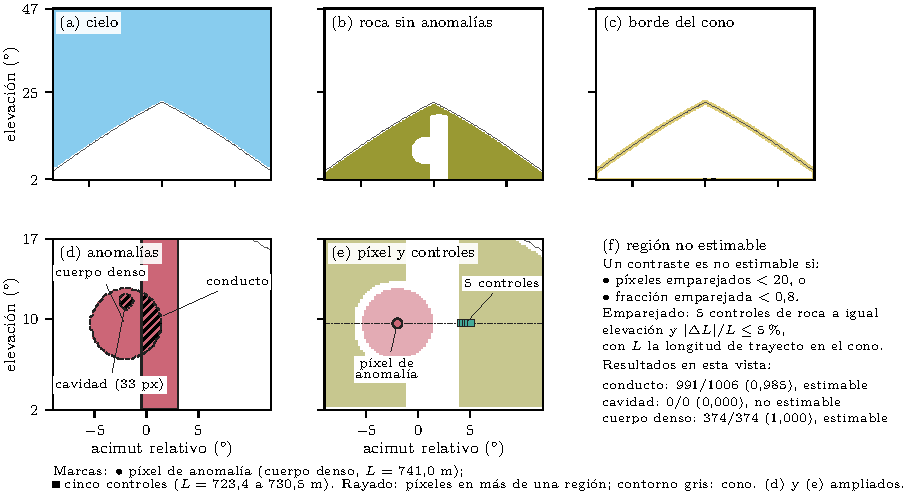
\includegraphics[width=\linewidth]{met_08_regiones_evaluacion.pdf}
\caption[Regiones y controles de evaluación]{Máscaras y controles en geo-train-08, vista 0. Los paneles de anomalías y controles amplían la región de interés. La cavidad no cumple el soporte emparejado en esta vista; se conserva como no estimable. Fuente: elaboración de los autores.}\label{fig:met-regiones}
\end{figure}
Se invirtieron predicciones a cuentas antes de sumar. Las Ecuaciones~\eqref{eq:met-sesgo} y~\eqref{eq:met-espacial} distinguen sesgo firmado y error espacial para región $R$ y realización $k$.
\begin{samepage}
\begin{subequations}
\begin{equation}b_{Rk}=\frac{\sum_{p\in R}(\widehat c_{kp}-c_p)}{\sum_{p\in R}c_p}.\label{eq:met-sesgo}\end{equation}
\begin{equation}a_{Rk}=\frac{\sum_{p\in R}|\widehat c_{kp}-c_p|}{\sum_{p\in R}c_p}.\label{eq:met-espacial}\end{equation}
\end{subequations}
\end{samepage}
El sesgo permite cancelación entre excesos y déficits; el error espacial acumula magnitudes. Se reportaron ambos para no identificar suma conservada con preservación espacial. Las regiones menores de veinte píxeles o con referencia nula se señalaron como no estimables mediante una regla común.

Las Ecuaciones~\eqref{eq:met-bmedio} y~\eqref{eq:met-q} definen $Q$. $\mathcal A_{gv}$ contiene anomalías elegibles y $V_g$ es el número de vistas; se exigió soporte completo.
\begin{samepage}
\begin{subequations}
\begin{equation}\overline b_{gvR}=\frac1{20}\sum_{k=1}^{20}b_{gvRk}.\label{eq:met-bmedio}\end{equation}
\begin{equation}Q_g=\frac1{V_g}\sum_v\frac12\left(|\overline b_{gv,\mathrm{roca}}|+\frac1{|\mathcal A_{gv}|}\sum_{a\in\mathcal A_{gv}}|\overline b_{gva}|\right).\label{eq:met-q}\end{equation}
\end{subequations}
\end{samepage}
El valor absoluto se aplicó después del promedio entre realizaciones. $Q$ no es error absoluto medio por píxel ni error de densidad. Sin anomalías o con soporte incompleto se conservó el indicador de roca y se señaló $Q$ como no aplicable o incompleto, sin asignarle cero.

\subsection{Contraste y corrección numérica}
Se comparó la media de cuentas de anomalía con controles de roca sin anomalía a igual elevación y trayectos próximos. Se excluyeron del núcleo objetivo los rayos que atravesaban otras anomalías, con margen de dos píxeles. Se exigió diferencia relativa de longitud no mayor de 0,05 y cinco controles por píxel, al menos veinte píxeles emparejados y cobertura mínima del 80\,\% del núcleo elegible. Los controles pudieron reutilizarse, ponderados por sus asignaciones a píxeles objetivo. No se interpretó este comparador como la misma escena sin anomalía, pues no se dispuso de ese contrafactual. Las Ecuaciones~\eqref{eq:met-contraste} y~\eqref{eq:met-error-contraste} definen contraste y error absoluto.
\begin{samepage}
\begin{subequations}
\begin{equation}\chi_R=\frac{\overline c_R}{\overline c_{\mathrm{control}(R)}}-1.\label{eq:met-contraste}\end{equation}
\begin{equation}E_{\chi,R}=|\widehat\chi_R-\chi_R^{\mathrm{ref}}|.\label{eq:met-error-contraste}\end{equation}
\end{subequations}
\end{samepage}
Se registraron controles nulos como no estimables. El resumen utilizó soporte común completo de todos los métodos, informando su tamaño y conservando otros casos en registros detallados. El contraste correspondió a cuentas, no a opacidad.

La revisión C2 corrigió la selección inestable de controles con longitudes prácticamente iguales. Las diferencias absolutas de longitud se ordenaron y agruparon desde el mínimo de cada grupo con tolerancia $10^{-8}$~m, sin encadenar empates transitivos; se desempató por columna. La tolerancia resolvió una cuestión numérica, no una resolución física. Se guardaron índices y huellas de máscaras para reproducir sin elegir controles nuevamente. Fue una corrección posterior a la evaluación y se identificó como tal; no cambió pesos, imágenes ni métricas de similitud.

\subsection{Agregación e interpretación}
Se informaron diferencias candidato menos comparador por geometría e indicador. Las comparaciones principales fueron cGAN frente a entrada, U-Net frente a entrada y cGAN frente a U-Net; las continuaciones se compararon dentro de cada pareja. No se eligió la mejor semilla con prueba. Las parejas compartieron pesos de partida y no estimaron variabilidad desde cero.

Se distinguieron soporte incompleto, ausencia de deterioro en los indicadores enumerados y compromiso o deterioro. Estas categorías fueron descriptivas: ausencia de deterioro no significó equivalencia estadística. No se usó mejora de SSIM para ocultar alteraciones de cuentas ni se trataron veinte realizaciones como veinte geometrías independientes. En EF-01 el alcance se limitó al catálogo y a la fracción del 5\,\%; el complemento multifracción se describe en la sección~\ref{sec:met-adquisicion}.

\section{Evaluación multifracción y métricas locales}\label{sec:met-adquisicion}
\subsection{Diseño del complemento y conservación de los modelos}
El análisis de adquisición se desarrolló en dos etapas. Primero se compararon las entradas sin red al 1, 5, 10 y 50\,\% con las redes evaluadas al 5\,\%. Esa comparación describió la relación entre estadística de conteo y calidad, pero no estableció un mínimo aceptable. Después se ejecutó el complemento OE3-C1, en el que los ocho modelos congelados recibieron las cuatro fracciones disponibles. Esta segunda etapa completó la evaluación experimental del tercer objetivo~\parencite{repositorioMuografia2026}.

Se mantuvieron las tres geometrías de prueba y la geometría de generalización, con seis vistas y veinte realizaciones por vista. Los modelos conservaron los pesos seleccionados o continuados al 5\,\%; no se entrenó una red distinta para cada fracción ni se ajustaron las pérdidas después de conocer la evaluación final. Por ello, la aplicación al 1, 10 y 50\,\% examinó la transferencia de los mismos modelos a otras estadísticas de entrada. Se distinguió expresamente esta evaluación de un entrenamiento multifracción.

La transformación de la Ecuación~\eqref{eq:met-entrada} se aplicó con la fracción de cada imagen y con la escala original. Se conservaron el modo de evaluación, lotes de cuatro imágenes, determinismo activado y TF32 desactivado. Se reutilizaron las 3\,840 predicciones al 5\,\%, previa comprobación de sus identidades, y se produjeron 11\,520 predicciones adicionales para las tres fracciones restantes. El conjunto evaluado comprendió así 15\,360 salidas de redes. Cada matriz mantuvo la correspondencia con geometría, vista, realización, fracción y modelo, necesaria para realizar comparaciones sobre las mismas referencias.

La Tabla~\ref{tab:met-complemento} resume el diseño. La Figura~\ref{fig:met-curvas} organiza la comparación multifracción y la aplicación del criterio de calidad; distingue los datos usados para entrenar de los utilizados exclusivamente para evaluar.
\begin{table}[htbp]\centering\small
\caption{Diseño de la evaluación multifracción OE3-C1.}\label{tab:met-complemento}
\begin{tabularx}{\linewidth}{@{}p{4.1cm}X@{}}\toprule
Elemento & Procedimiento establecido\\\midrule
Modelos & U-Net y cGAN originales; seis continuaciones E1 B1--B3, C0/C1.\\
Fracciones & 0,01; 0,05; 0,10; 0,50, con los mismos pesos entrenados al 5\,\%.\\
Entradas por fracción & 360 de prueba y 120 de generalización.\\
Referencia & La imagen finita de alta estadística de la misma vista.\\
Comparador sin red & Conteos divididos por la fracción y transformados con la escala original.\\
Criterio principal & Alcanzar conjuntamente SSIM y PSNR de la entrada sin red al 50\,\%, en todas las vistas de cada partición.\\
Análisis local & Cuentas regionales, SNR espacial, CNR firmado, contraste e inversiones de signo.\\\bottomrule
\end{tabularx}\end{table}
\FiguraPendienteMet{met_09_evaluacion_multifraccion}{Diseño de la evaluación multifracción y del criterio de reducción. El sesgo regional se promedia entre realizaciones antes de construir $Q$; este indicador no interviene en el criterio conjunto de SSIM y PSNR.}{fig:met-curvas}{Reemplazar el esquema histórico met\_09, que muestra redes solo al 5 por ciento. Dibujar cuatro columnas de entrada: 1, 5, 10 y 50 por ciento; cada una alimenta los mismos ocho modelos congelados. Mostrar T(L/f), sin reajustar s, y una referencia C común. Separar entrenamiento al 5 por ciento de evaluación en cuatro fracciones. Indicar 3840 predicciones reutilizadas y 11520 nuevas. Conectar las métricas por realización con promedios de veinte realizaciones por vista. Dibujar dos condiciones simultáneas, SSIM y PSNR frente a entrada sin red al 50 por ciento, y exigir todas las vistas dentro de cada partición. Si hay fracciones aceptadas, calcular mínimo y R=0,50/f mínimo; si no las hay, informar no determinado. No incluir resultados ni simular curvas. Entregar esquema vectorial legible y fuente editable.}

\subsection{Indicadores locales de anomalía y fondo}\label{subsec:met-locales}
Se conservaron las máscaras geométricas y los índices de controles estabilizados en C2. Para cada anomalía se identificaron los píxeles objetivo emparejados y sus cinco controles por píxel. La media de fondo conservó las ponderaciones derivadas de esas asignaciones. Para calcular su desviación espacial se empleó, en cambio, el conjunto de donantes únicos; de esta forma, la reutilización de un mismo píxel como control no se interpretó como una observación adicional para estimar dispersión.

Las Ecuaciones~\eqref{eq:met-snrlocal} y~\eqref{eq:met-cnrlocal} definen los indicadores de intensidad respecto de dispersión espacial y de contraste respecto del fondo. Se aplicaron a la referencia, a las entradas escaladas y a las cuentas recuperadas de cada red.
\begin{samepage}\begin{subequations}
\begin{equation}\operatorname{SNR}_{A}=\frac{\mu_A}{s_A}.\label{eq:met-snrlocal}\end{equation}
\begin{equation}\operatorname{CNR}_{A,B}=\frac{\mu_A-\mu_B}{s_B}.\label{eq:met-cnrlocal}\end{equation}
\end{subequations}\end{samepage}
Aquí $\mu_A$ es la media de cuentas de los objetivos emparejados, $\mu_B$ la media ponderada de los controles, y $s_A$ y $s_B$ sus desviaciones espaciales, calculadas con corrección de un grado de libertad. El contraste de cuentas se conservó como en la Ecuación~\eqref{eq:met-contraste}. Las tres magnitudes son adimensionales, pero responden a preguntas diferentes: SNR mide intensidad relativa a heterogeneidad interna; CNR conserva el signo de la diferencia respecto del fondo; el contraste expresa esa diferencia en relación con la media del fondo.

La dispersión espacial puede contener tanto fluctuación de conteo como estructura de la escena. En consecuencia, un SNR elevado no se interpretó automáticamente como mayor detectabilidad. Una salida suavizada puede reducir la dispersión y elevar el cociente aunque atenúe una anomalía. La lectura de estos indicadores se acompañó del error de contraste, de su signo y de los errores regionales, sin adoptar un umbral universal de detección.

Se registró también la variabilidad entre realizaciones mediante las Ecuaciones~\eqref{eq:met-dreal} y~\eqref{eq:met-snrrep}. Para una misma anomalía y vista, $k$ identifica las veinte realizaciones y $s_k$ su desviación muestral.
\begin{samepage}\begin{subequations}
\begin{equation}D_k=\mu_{A,k}-\mu_{B,k}.\label{eq:met-dreal}\end{equation}
\begin{equation}J_{\mathrm{rep}}=\frac{\overline D}{s_k(D_k)}.\label{eq:met-snrrep}\end{equation}
\end{subequations}\end{samepage}
Este cociente no se dividió por la raíz del número de realizaciones ni se interpretó como estadístico de significación. La referencia única no proporciona veinte realizaciones independientes para calcularlo. Cuando la desviación fue nula o el soporte insuficiente se conservó el motivo de no estimabilidad, sin asignar infinito ni éxito automático.

Se mantuvieron al menos veinte píxeles objetivo emparejados y cobertura mínima del 80\,\% del núcleo elegible. Para cada indicador se verificaron los denominadores y la finitud. No se añadieron pseudocuentas ni se sustituyeron valores no estimables por cero. Los soportes comunes se construyeron por métrica para comparar exactamente los mismos casos entre métodos y fracciones.

\subsection{Agregación de errores y conservación del signo}
Los errores locales se calcularon respecto de la misma referencia antes de promediar. La Ecuación~\eqref{eq:met-errorlocal} define el error para un indicador $M$, una combinación $a$ de anomalía y vista y la realización $k$. La Ecuación~\eqref{eq:met-signo} identifica una inversión de signo del contraste.
\begin{samepage}\begin{subequations}
\begin{equation}e_{ak}^{(M)}=\left|M_{ak}^{\mathrm{met}}-M_a^{\mathrm{ref}}\right|.\label{eq:met-errorlocal}\end{equation}
\begin{equation}I_{ak}^{\mathrm{signo}}=\mathbf1\!\left\{C_{N,ak}^{\mathrm{met}}C_{N,a}^{\mathrm{ref}}<0\right\}.\label{eq:met-signo}\end{equation}
\end{subequations}\end{samepage}
En la segunda expresión se emplea $C_N$ para el contraste de cuentas definido anteriormente como $\chi_R$. El producto estrictamente negativo exige signos opuestos; los ceros no se cuentan como inversiones. No se eliminó una referencia por tener contraste próximo a cero, aunque se reconoció la sensibilidad de la clasificación en ese caso.

Se promediaron errores sobre realizaciones, luego sobre los casos elegibles de cada geometría y finalmente entre geometrías, con igual peso dentro de la partición. Prueba y generalización permanecieron separadas. El soporte común de SNR comprendió diecinueve combinaciones en prueba y once en generalización; para CNR y contraste fueron veintiuna y once. SSIM, PSNR y $Q$ se mantuvieron sobre sus propios soportes y no se filtraron mediante las exclusiones locales.

Este orden es necesario para interpretar las tablas: el promedio de errores absolutos no equivale al error del promedio. Por ello, el contraste local del complemento no se mezcló con el resumen histórico C2, que utilizó otro soporte y otra agregación. Se conservaron ambos registros con su definición y procedencia.

\section{Criterio de reducción y diagnóstico de opacidad}\label{sec:met-factor}
\subsection{Exposición convencional y comparación operativa}
Bajo flujo estable y detección constante, la esperanza del conteo es proporcional al tiempo. Las Ecuaciones~\eqref{eq:met-tiempo} y~\eqref{eq:met-razon} expresan esa hipótesis y la razón nominal entre fracciones.
\begin{samepage}\begin{subequations}
\begin{equation}\mathbb E[N(t)]=\lambda t.\label{eq:met-tiempo}\end{equation}
\begin{equation}R_{\mathrm{nom}}=\frac{f_{\mathrm{comparador}}}{f_{\mathrm{modelo}}}.\label{eq:met-razon}\end{equation}
\end{subequations}\end{samepage}
La tasa $\lambda$ se supone constante. La razón corresponde a conteos esperados bajo esas condiciones; no representa un tiempo medido en campo. La campaña conservó además la etiqueta convencional de la Ecuación~\eqref{eq:met-exposicion}, donde $N^{\mathrm{nom}}_{gv}$ identifica los primarios de la ventana nominal y $S_0$ es la normalización tabulada de 36\,034\,069,911914065 cuentas.
\begin{equation}T^{\mathrm{conv}}_{gv}=30\,\mathrm d_{\mathrm{conv}}\frac{N^{\mathrm{nom}}_{gv}}{S_0}.\label{eq:met-exposicion}\end{equation}
La etiqueta en días convencionales no constituyó una calibración temporal de un detector. Del mismo modo, dividir por 0,05 produce una razón nominal de veinte respecto de la referencia completa, pero no establece la calidad de la imagen obtenida con una red.

El complemento adoptó como referente operativo la entrada sin red al 50\,\%, por ser el mayor nivel disponible distinto de la referencia completa. Para cada vista se calcularon sus promedios de SSIM y PSNR sobre veinte realizaciones frente a la referencia. Se conservaron los 48 umbrales resultantes antes de ejecutar las nuevas inferencias. Este criterio evitó utilizar la comparación de la referencia consigo misma, cuyo PSNR sería infinito.

La regla se fijó después de conocer los resultados históricos al 5\,\% y las curvas de entrada. Por tanto, fue previa a las nuevas inferencias, pero no un umbral original de la propuesta ni una validación confirmatoria independiente. Su carácter operativo se mantuvo separado de una aceptación geofísica. Las métricas regionales y locales se discutieron como evidencia complementaria, sin sustituir retrospectivamente el criterio principal cuando su resultado fue desfavorable.

\subsection{Fracción mínima y factor asociado}\label{subsec:met-minimo}
Las Ecuaciones~\eqref{eq:met-umbral-s} y~\eqref{eq:met-umbral-p} definen los umbrales por vista $v$. Las barras indican promedio entre las veinte realizaciones y todas las comparaciones se realizan frente a la misma referencia de alta estadística.
\begin{samepage}\begin{subequations}
\begin{equation}\tau_{S,v}=\overline{\operatorname{SSIM}}_{\mathrm{entrada},0{,}50,v}.\label{eq:met-umbral-s}\end{equation}
\begin{equation}\tau_{P,v}=\overline{\operatorname{PSNR}}_{\mathrm{entrada},0{,}50,v}.\label{eq:met-umbral-p}\end{equation}
\end{subequations}\end{samepage}
Para cada modelo $m$ y partición $S$, se exigió que ambas métricas alcanzaran sus umbrales en todas las vistas. La Ecuación~\eqref{eq:met-aceptadas} expresa el conjunto de fracciones aceptadas, con $F=\{0{,}01;0{,}05;0{,}10;0{,}50\}$ y tolerancia exclusivamente aritmética $\varepsilon=10^{-12}$.
\begin{equation}
\mathcal A_{m,S}=\left\{f\in F:\ \forall v\in S,\
\begin{array}{l}\overline{\operatorname{SSIM}}_{m,f,v}+\varepsilon\geq\tau_{S,v}\\
\overline{\operatorname{PSNR}}_{m,f,v}+\varepsilon\geq\tau_{P,v}\end{array}\right\}.
\label{eq:met-aceptadas}\end{equation}
La tolerancia no fue un margen de equivalencia de calidad. Cuando el conjunto no es vacío, las Ecuaciones~\eqref{eq:met-fmin} y~\eqref{eq:met-factor} definen el mínimo muestreado y la razón asociada al referente del 50\,\%.
\begin{samepage}\begin{subequations}
\begin{equation}f_{\min,m,S}=\min\mathcal A_{m,S}.\label{eq:met-fmin}\end{equation}
\begin{equation}R_{m,S}=\frac{0{,}50}{f_{\min,m,S}}.\label{eq:met-factor}\end{equation}
\end{subequations}\end{samepage}
Si el conjunto es vacío, ambas cantidades se informan como no determinadas. No se asigna cero ni uno, ni se interpola un valor entre las fracciones. Se examinó toda la rejilla sin suponer monotonía. El Algoritmo~\ref{alg:met-factor} resume la decisión y conserva por separado las dos particiones.
\begin{algorithm}[htbp]\small
\caption{Evaluación de la fracción mínima en la rejilla disponible.}\label{alg:met-factor}
\begin{algorithmic}[1]
\Require Métricas por realización, pesos congelados y umbrales por vista.
\Ensure Conjuntos aceptados y factores determinados o no determinados.
\For{cada modelo y cada partición}
\State Inicializar el conjunto de fracciones aceptadas como vacío.
\For{cada fracción de la rejilla}
\State Promediar SSIM y PSNR por vista sobre veinte realizaciones.
\If{ambas métricas alcanzan sus umbrales en todas las vistas}
\State Incorporar la fracción al conjunto aceptado.
\EndIf
\EndFor
\If{el conjunto aceptado está vacío}
\State Registrar mínimo y factor como no determinados.
\Else
\State Obtener el mínimo y calcular la razón respecto de 0,50.
\EndIf
\State Conservar todas las comparaciones y las exclusiones.
\EndFor
\end{algorithmic}\end{algorithm}

\subsection{Opacidad nominal y controles geométricos}\label{sec:met-opacidad}
Como complemento de la interpretación, se calculó una referencia geométrica de opacidad a partir del catálogo y de los rayos centrales. La Ecuación~\eqref{eq:met-opacidad} expresa la integral de densidad a lo largo de una trayectoria. Para una trayectoria recta de longitud total $L$ que atraviesa una sola anomalía durante una longitud $\ell$, la Ecuación~\eqref{eq:met-opacidadnom} define la opacidad nominal utilizada.
\begin{samepage}\begin{subequations}
\begin{equation}X=\int\rho(l)\,\mathrm dl.\label{eq:met-opacidad}\end{equation}
\begin{equation}X_{\mathrm{nom}}=100\left[\rho_r(L-\ell)+\rho_a\ell\right].\label{eq:met-opacidadnom}\end{equation}
\end{subequations}\end{samepage}
Las densidades $\rho_r$ y $\rho_a$ se expresan en g\,cm$^{-3}$ y las longitudes en metros; el factor cien convierte estas últimas a centímetros, de modo que $X$ queda en g\,cm$^{-2}$. Esta magnitud no se identificó con el contraste adimensional de cuentas.

Se conservaron las máscaras y los controles C2. Se comprobó que los objetivos seleccionados no atravesaran otras anomalías y que los controles no atravesaran anomalías, evitando sumar materiales incompatibles en regiones superpuestas. La diferencia entre opacidad media de objetivo y control se separó como en la Ecuación~\eqref{eq:met-opacidaddelta}.
\begin{equation}\overline X_A-\overline X_B=100(\rho_a-\rho_r)\overline\ell+100\rho_r(\overline L_A-\overline L_B).\label{eq:met-opacidaddelta}\end{equation}
El primer término describe el contraste nominal de densidad y el segundo la diferencia de longitud entre los rayos comparados. Se preservaron las ponderaciones de los controles y se verificaron unidades y composición mediante casos analíticos. Así se evitó atribuir a la anomalía una diferencia causada únicamente por trayectos distintos.

El cálculo utilizó densidades declaradas y trayectorias rectas; no reconstruyó opacidad desde las predicciones ni siguió las trayectorias dispersadas de los muones. Se registró la discrepancia de material de la anomalía 2 de \texttt{geo-gen-01}, cuya densidad nominal de 0,048~g\,cm$^{-3}$ activa la sustitución por aire en el constructor conservado. No se supuso una densidad efectiva de producción sin trazabilidad del entorno ejecutado. Este diagnóstico delimitó la interpretación de las métricas, sin modificar las imágenes, sus referencias ni los criterios del experimento cerrado.


\section{Reproducibilidad y trazabilidad}\label{sec:met-reproducibilidad}
Se conservaron catálogo, tablas, receta, semillas, coordenadas, particiones, escala, pesos y predicciones con identidades verificables. Una huella comprobó igualdad de archivos; no se interpretó como prueba de validez científica ni del momento en que se tomó una decisión.

Se distinguieron tres niveles: integridad y correspondencia; recálculo de transformaciones y métricas desde matrices; y nueva ejecución de un procedimiento, como recuperación o inferencia desde pesos. El recálculo de métricas no se describió como repetición completa de transporte o entrenamiento.

La Tabla~\ref{tab:met-trazabilidad} resume los elementos mínimos. Las fuentes detalladas se conservaron en la revisión documental \texttt{9558099}~\parencite{repositorioMuografia2026}. Los comandos y registros extensos permanecieron como material reproducible; el capítulo describió operaciones en lenguaje metodológico y pseudocódigo.
\begin{table}[htbp]\centering\small
\caption{Información para reproducir e interpretar la cadena.}\label{tab:met-trazabilidad}
\begin{tabularx}{\linewidth}{@{}p{2.7cm}XX@{}}\toprule
Etapa & Identidad mínima & Comprobación\\\midrule
Transporte & Receta, entorno, binario, geometrías, tablas y semillas. & Bloques, primarios, coordenadas y sumas.\\
Preparación & Referencias, fracciones, semillas y versión de NumPy. & Correspondencia de arreglos y procedencia.\\
Entrenamiento & Particiones, escala, código, optimizadores y estados aleatorios. & Recuperación y rechazo de identidades incompatibles.\\
Evaluación & Pesos, orden de imágenes, máscaras y controles C2. & Integridad y recálculo de métricas.\\
Adquisición & Fracciones, soporte y supuestos temporales. & Comparación discreta sin extrapolación.\\\bottomrule
\end{tabularx}\end{table}
La producción Geant4 correspondió a ejecuciones estudiantiles en SC3. Los entrenamientos conservaron el entorno de cada entrega, sin atribuirlos automáticamente al de transporte. La reproducción local de pares registró NumPy~2.4.4; la revisión C2 utilizó Python~3.12.14, NumPy~2.3.5, PyTorch~2.6.0 y scikit-image~0.26.0. Son versiones de etapas diferentes, no un entorno universal.

Las limitaciones se incorporaron al diseño de interpretación: geometrías idealizadas, fuente híbrida, registro de primarios, referencia finita, dependencia entre realizaciones, exposición histórica de escenas y entrenamiento de redes en una sola fracción. Estas condiciones delimitan lo que puede concluirse. El criterio operativo de comparación se aplicó a toda la rejilla de fracciones y se conservó su resultado, incluso cuando no permitió definir un factor. El cierre experimental no implicó equivalencia instrumental ni reconstrucción cuantitativa de opacidad.
\FloatBarrier

